Generative stochastic networks (GSN) are a generalization of the denoising auto-encoder and help solve the problem of mixing between many major modes of the input data distribution.

\subsection{Denoising auto-encoder}
Denoising auto-encoders use a Markov chain to learn a reconstruction distribution \(P(X|\widetilde{X})\) given a corruption process \(C(\widetilde{X}|X)\) for some data \(X\). Denoising auto-encoders have been shown as generative models \cite{bengio13a}, where the Markov chain can be iteratively sampled from:
\begin{equation}
	X_t \sim P_\Theta(X|\widetilde{X}_{t-1})
\end{equation}
\begin{equation}
	\widetilde{X}_t \sim C(\widetilde{X}|X_t)
\end{equation}
As long as the learned distribution \(P_{\Theta_n}(X|\widetilde{X})\) is a consistent estimator of the true conditional distribution \(P(X|\widetilde{X})\) and the Markov chain is ergodic, then as \(n \rightarrow \infty\), the asymptotic distribution \(\pi_n(X)\) of the generated samples from the denoising auto-encoder converges to the data-generating distribution \(P(X)\) \cite{bengio13a}). 


\subsection{Easing restrictive conditions on the denoising auto-encoder}

A few restrictive conditions are necessary to guarantee ergodicity of the Markov chain - requiring \(C(\widetilde{X}|X) > 0\) everywhere that \(P(X) > 0\). Particularly, a large region \(V\) containing any possible \(X\) is defined such that the probability of moving between any two points in a single jump \(C(\widetilde{X}|X)\) must be greater than 0. This restriction requires that \(P_{\Theta_n}(X|\widetilde{X})\) has the ability to model every mode of \(P(X)\), which is a problem this model was meant to avoid.

To ease this restriction, Bengio et al. \cite{gsn} prove that using a \(C(\widetilde{X}|X)\) that only makes small jumps allows \(P_{\Theta}(X|\widetilde{X})\) to model a small part of the space \(V\) around each \(\widetilde{X}\). This weaker condition means that modeling the reconstruction distribution \(P(X|\widetilde{X})\) would be easier since it would probably have fewer modes. 

However, the jump size \(\sigma\) between points must still be large enough to guarantee that one can jump often enough between the major modes of \(P(X)\) to overcome the regions of low probability: \(\sigma\) must be larger than half the largest distance of low probability between two nearby modes, such that \(V\) has at least a single connected component between modes. This presents a tradeoff between the difficulty of learning \(P_{\Theta}(X|\widetilde{X})\) and the ease of mixing between modes separated by this low probability region.


\subsection{Generalizing to GSN}

While denoising auto-encoders can rely on \(X_t\) alone through a deterministic procedure for the state of the Markov chain, GSNs introduce a latent variable \(H_t\) that acts as an additional state variable in the Markov chain along with the visible \(X_t\) \cite{gsn}:
\begin{equation}
	H_{t+1} \sim P_{\Theta_1}(H|H_t, X_t)
\end{equation}
\begin{equation}
	X_{t+1} \sim  P_{\Theta_2}(X|H_{t+1})
\end{equation}

The resulting computational graph is shown in Figure \ref{fig:gsn}.
\begin{figure}[h!]
  \centering
    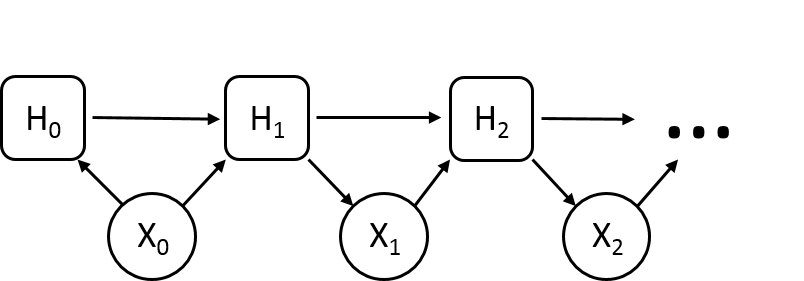
\includegraphics[width=0.3\textwidth]{gsn_computational_graph}
\caption{GSN computational graph.}\label{fig:gsn}
\end{figure}

The latent state variable \(H\) can be equivalently defined as \(H_{t+1} = f_{\Theta_1}(X_t,Z_t,H_t)\), a learned function \(f\) with an independent noise source \(Z_t\) such that \(X_t\) cannot be reconstructed exactly from \(H_{t+1}\). If \(X_t\) could be recovered from \(H_{t+1}\), the reconstruction distribution would simply converge to the Dirac at \(X\). Denoising auto-encoders are therefore a special case of GSNs, where \(f\) is fixed instead of learned.

GSNs also use the notion of walkbacks to aid training. Walkbacks are the process of generating samples by iteratively sampling from \(P_{\Theta_1}(H|H_t, X_t)\) and \(P_{\Theta_2}(X|H_{t+1})\) for a given input. By using walkbacks, the model is more likely to seek out spurious modes in the data distribution and correct for them \cite{bengio13a}. The resulting Markov chain of a GSN is inspired by Gibbs sampling, but with stochastic units at each layer that can be backpropagated \cite{rezende14}.

\begin{figure}[h!]
  \centering
    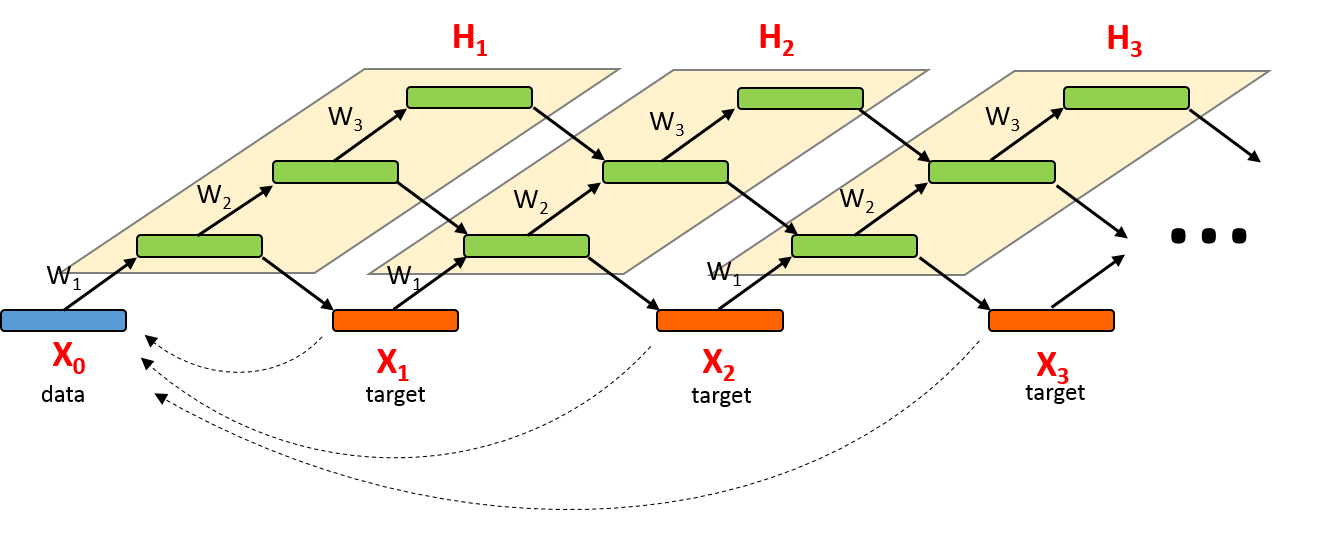
\includegraphics[width=0.5\textwidth]{gsn_markov_chain}
\caption{Unrolled GSN Markov chain.}
\end{figure}

Experimental results with GSNs show that their latent states mix well between the major modes of the data - mixing faster at higher layers in the model \cite{gsn}. Using this property, we tested a simple temporal GSN model to predict sequences of inputs. The temporal GSN uses a linear transformation \(H \rightarrow H\) to predict \(P(H_t|H_{t-1},...,H_{t-n})\) with an input history of size \(n\). Using this predicted \(H_t\), an expected input \(x_t\) was sampled from the model's learned reconstuction distribution \(P_{\Theta_2}(X|H)\).

Qualitatively, this model appears to predict temporal dependencies well within its history window \(n\) (Figure \ref{fig:tgsn}). This result provided motivation to use the latent state \(H\) as the emitted parameter in a better-suited temporal model, such as an RNN.

\begin{figure}[h!]
  \centering
    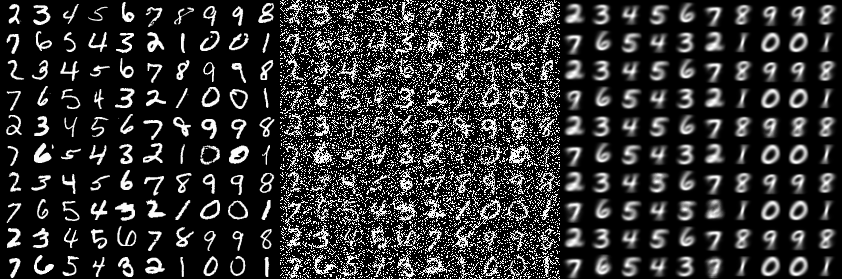
\includegraphics[width=0.5\textwidth]{tgsn}
\caption{Temporal GSN with history \(n=2\) trained on an arbitrary MNIST sequence. Original input sequence is on the left, a noisy version of the input fed into the model is in the middle, and the predicted input based on the history is on the right.}\label{fig:tgsn}
\end{figure}